\section{Esempi di lavorazione}
Mostriamo ora alcuni esempi di lavorazione, per vedere come i tempi di esecuzione catalogati variano a seconda dei parametri scelti.

Le prove sono state effettuate usando i due file messi a disposizione per i testing, chiamati \texttt{positions.txt} e \texttt{positions2.txt}. Il primo file contiene oltre $7000$ posizioni, e riproduce una fresatura limitata ad una ristretta porzione di blocco, generando quindi un Octree poco bilanciato. Il secondo file invece contiene oltre $20000$ posizioni e riproduce una fresatura che scava ``tutto attorno'' al blocco, generando quindi un Octree più bilanciato e risultando quindi più onerosa dal punto di vista della computazione. In \ref{tab:lavfinali} vediamo il risultato delle due lavorazioni.
\begin{center}
\begin{table}[h]
  \begin{tabular}{cc}
   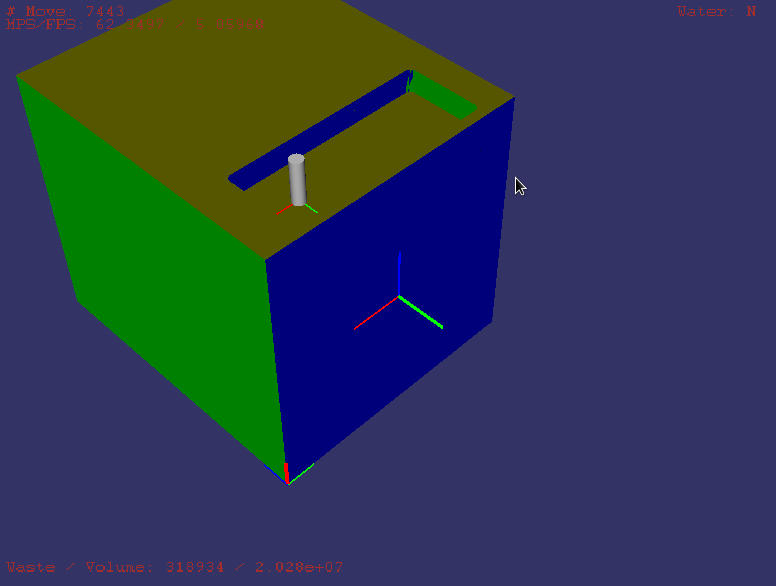
\includegraphics[width=0.48\textwidth]{img/screenshots/pos_box_v05_1.png} &%
   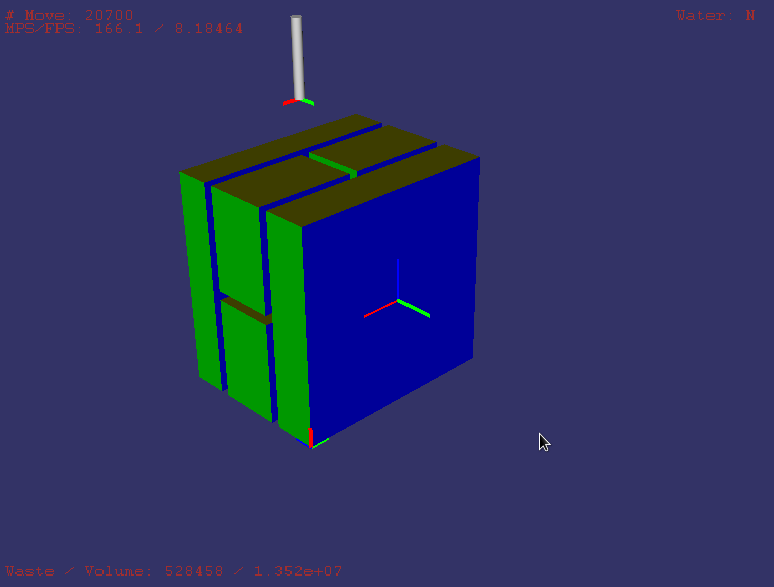
\includegraphics[width=0.48\textwidth]{img/screenshots/pos2_box_v1_2.png}\\
  \end{tabular}
  \caption{Risultato delle lavorazioni contenute nei file \texttt{positions.txt} e \texttt{positions2.txt}.}
  \label{tab:lavfinali}
\end{table}
\end{center}
I tempi riportati si riferiscono a test effettuati usando una macchina con Ubuntu Linux 12.04 a 64 bit, con processore Intel i7 a 1.73 GHz e 4GB di RAM, con il simulatore compilato in modalità \verb!release! e lanciato, salvo dove indicato, per completare la lavorazione alla massima velocità possibile. Per il profiling invece si è reso necessario compilare on modalità \verb!debug!. Abbiamo effettuato varie prove per ciascuna configurazione, e abbiamo qui riportato i valori mediani.

\subsection{Modalità testuale}
Vediamo innanzitutto% (tabelle \ref{tab:positionsnone} e \ref{tab:positions2none})
(tabella \ref{tab:graphicsnone}) come si comporta il simulatore quando viene eseguito in modalità solo testuale.
\begin{center}
  \begin{table}[h]
       \centering
      \begin{tabular}{cccccc}
        \toprule
        & \multicolumn{2}{c}{file \texttt{positions.txt}} & & \multicolumn{2}{c}{file \texttt{positions2.txt}}\\
        \cmidrule(r){2-3}\cmidrule(r){5-6}
          \shortstack{Dimensione\\ Voxel} & \shortstack{Tempo \\\texttt{[s]}} & \shortstack{Memoria \\\texttt{[MB]}} & & \shortstack{Tempo \\\texttt{[s]}} & \shortstack{Memoria \\\texttt{[MB]}}\\
        \midrule
          3   & 0.517  & -     & & 2.446   & 22.7   \\
          2.5 & 0.543  & -     & & 2.558   & 12.2   \\
          2   & 1.632  & 17.2  & & 11.478  & 90.6   \\
          1.5 & 1.607  & -     & & 11.613  & 95.0   \\
          1   & 8.437  & 70.0  & & 99.785  & 463.4  \\
          0.5 & 67.691 & 334.7 & & 973.191 & 2764.8 \\
        \bottomrule
      \end{tabular}
      \caption{Riepilogo dei test effettuati in modalità testuale.}
      \label{tab:graphicsnone}
  \end{table}
\end{center}
Vediamo come con voxel grandi i tempi di esecuzione sono molto ridotti e molto simili, mentre con voxel più piccoli i tempi crescono compatibilmente con un fattore 8 (l'arietà dell'Octree). La mancanza di alcuni valori di memoria in tabella è causata dal fatto che la lavorazione contenuta nel file \texttt{positions.txt} con voxel grandi termina prima che sia possibile leggere la quantità di RAM occupata. Osservando però i valori rilevati per lo stesso file con voxel più piccoli, e paragonandoli con i valori osservati nella lavorazione riportata nel file \texttt{positions2.txt} possiamo inferire che l'occupazione si limita a pochi \texttt{MB}.

Questo è segno che con voxel grandi l'albero generato è poco profondo e viene analizzato molto velocemente, con un impatto poco significativo sul tempo di esecuzione totale. Al diminuire della dimensione dei voxel, l'Octree è invece più profondo, e la sua scansione occupa una parte sempre più consistente del tempo di esecuzione totale.

Per quanto riguarda i tempi rilevati per la lavorazione del file \texttt{positions2.txt} con dimensione voxel pari a $0.5$, si segnala che la lavorazione è stata rallentata dalle operazioni di swap occorse a causa dell'elevata quantità di memoria richiesta.

\subsection{Modalità grafica \texttt{box}}
La modalità grafica \texttt{box} è la modalità che non utilizza l'algoritmo Marching Cubes per il taglio dei voxel, ma usa l'oggetto \texttt{Box} di OpenSceneGraph per rappresentare ciascun voxel. Il risultato sarà l'esecuzione dell'interfaccia grafica di OSG per la visualizzazione delle varie fasi della lavorazione, con il rendering della lavorazione mediante cubi di varie dimensioni che rappresentano i voxel dell'Octree.

\subsection{Modalità grafica \texttt{mesh}}
La terza modalità di visualizzazione è quella che utilizza l'algoritmo Marching Cubes per estrarre la mesh tridimensionale dai voxel. Come nella modalità \texttt{box}, anche in questo caso viene lanciato il visualizzatore di OSG, ma la lavorazione viene resa in maniera più precisa mediante l'approssimazione calcolata da Marching Cubes (vedasi sezione \ref{mcalgo}) nel modulo Mesher a partire dai voxel. Un confronto tra le due modalità viene effettuato nella sezione successiva.

\subsection{Confronto tra \texttt{box} e \texttt{mesh}}
Mettiamo ora a confronto la visualizzazione della lavorazione con la modalità di visualizzazione \texttt{box} e la modalità \texttt{mesh} (le immagini sono zoomate per apprezzare le differenze).
\begin{center}
\begin{table}[hbtp]
  \begin{tabular}{cc}
   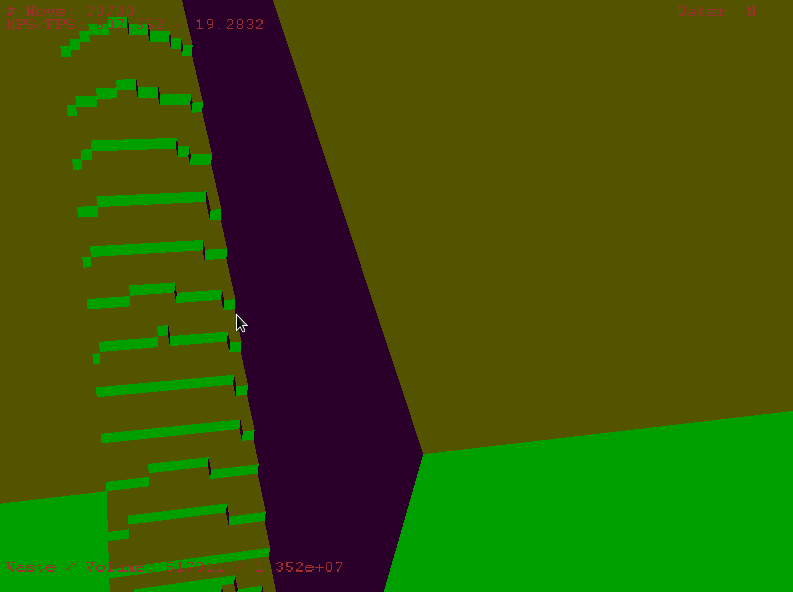
\includegraphics[width=0.48\textwidth]{img/screenshots/pos2_box_v2_2.png} &%
   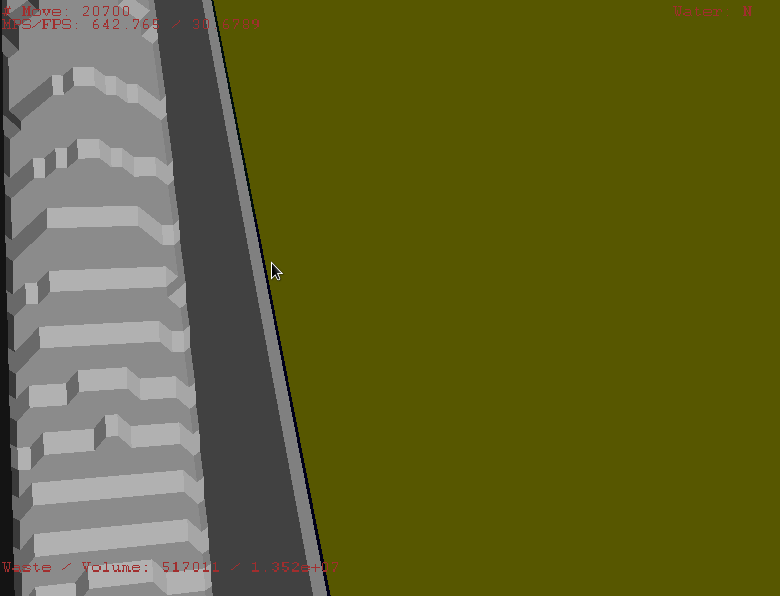
\includegraphics[width=0.48\textwidth]{img/screenshots/pos2_mesh_v2_2.png}\\
  \end{tabular}
  \caption{Confronto tra modalità \texttt{box} e modalità \texttt{mesh} con dim. voxel pari a $2$.}
  \label{tab:confrontobm1}
\end{table}
\end{center}

\begin{center}
\begin{table}[hbtp]
  \begin{tabular}{cc}
   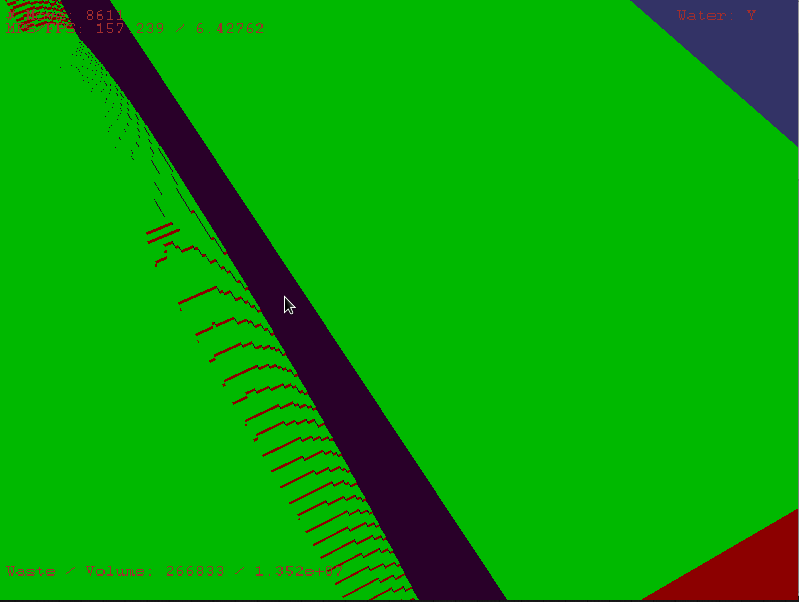
\includegraphics[width=0.48\textwidth]{img/screenshots/pos2_box_v1.png} &%
   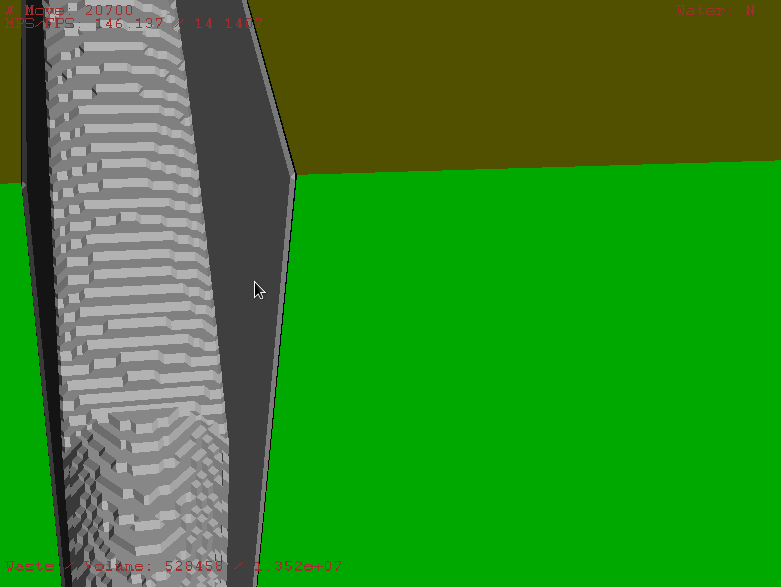
\includegraphics[width=0.48\textwidth]{img/screenshots/pos2_mesh_v1_2.png}\\
  \end{tabular}
  \caption{Confronto tra modalità \texttt{box} e modalità \texttt{mesh} con dim. voxel pari a $1$.}
  \label{tab:confrontobm2}
\end{table}
\end{center}

\begin{center}
\begin{table}[hbtp]
  \begin{tabular}{cc}
   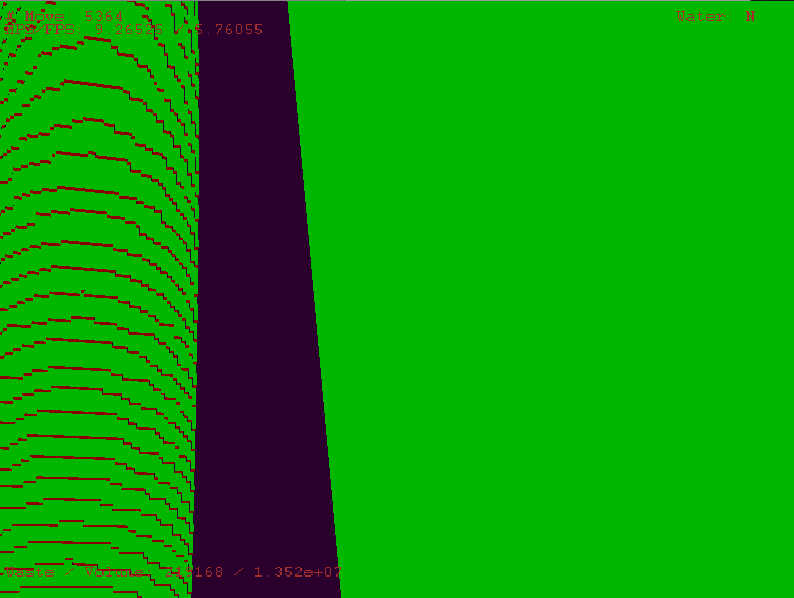
\includegraphics[width=0.48\textwidth]{img/screenshots/pos2_box_v05.png} &%
   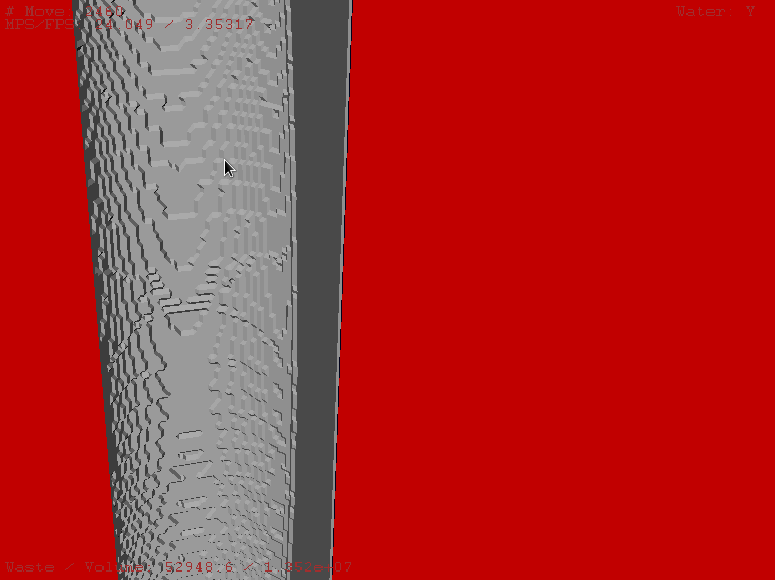
\includegraphics[width=0.48\textwidth]{img/screenshots/pos2_mesh_v05.png}\\
  \end{tabular}
  \caption{Confronto tra modalità \texttt{box} e modalità \texttt{mesh} con dim. voxel pari a $0.5$.}
  \label{tab:confrontobm3}
\end{table}
\end{center}

In \ref{tab:confrontobm1} vediamo la differenza nell'approssimazione della fresatura da parte del cilindro in modalità \texttt{box} (a sx) e \texttt{mesh} (a dx) con dimensione minima dei voxel pari a $2$. Vediamo come, nella modalità \texttt{mesh}, l'algoritmo Marching Cubes approssimi meglio la lavorazione, pur mantenendo visibile la struttura ``a cubi'' del rendering.

In \ref{tab:confrontobm2} e \ref{tab:confrontobm3} invece vediamo la stessa lavorazione, effettuata con dimensione dei voxel pari a, rispettivamente, $1$ e $0.5$. Vediamo come man mano che la dimensione dei voxel diminuisce, entrambe le modalità, ovviamente, approssimano in maniera sempre più precisa la fresatura. Tuttavia, mentre la modalità \texttt{box} approssima la lavorazione in modo sempre più preciso ma rimane comunque visibile la quadrettatura, l'algoritmo Marching Cubes che lavora alla stessa profondità dell'Octree fornisce risultati sempre più precisi e realistici.

Vediamo invece dalla tabella \ref{tab:confrontoBoxMesh} come l'implementazione con Marching Cubes possa risultare competitiva rispetto alla mera visualizzazione di cubi in lavorazioni brevi e che comportino la generazione di un Octree poco bilanciato e poco profondo. All'aumentare della profondità dell'albero, invece, la semplicità della generazione dei \texttt{Box} di OSG risulta più veloce. Per lavorazioni più complesse, che richiedono un Octree più completo, l'approccio \texttt{box} è più veloce rispetto alla generazione della \texttt{mesh} in tutti i test effettuati.

Segnaliamo che, per dimensioni minime dei voxel sufficientemente grandi, la lavorazione termina in tempi talmente brevi che risulta impossibile misurare un tempo attendibile. Inoltre, i tempi per le lavorazioni con Octree più profondo sono da considerarsi al netto del tempo di swap, che può essere più o meno consistente a seconda della quantità di memoria RAM a disposizione.

\begin{center}
  \begin{table}[hb]
   \centering
      \begin{tabular}{cccccc}
        \toprule
        & \multicolumn{2}{c}{file \texttt{positions.txt}} & & \multicolumn{2}{c}{file \texttt{positions2.txt}}\\
        \cmidrule(r){2-3}\cmidrule(r){5-6}
          \shortstack{Dimensione\\ Voxel} & \shortstack{Tempo \\con \texttt{box} \texttt{[s]}} & \shortstack{Tempo \\con \texttt{mesh} \texttt{[s]}} & & \shortstack{Tempo \\con \texttt{box} \texttt{[s]}} & \shortstack{Tempo \\con \texttt{mesh} \texttt{[s]}}\\
        \midrule
          3   & -      & -      & & 2.381    & 2.690    \\
          2.5 & -      & -      & & 2.510    & 2.581    \\
          2   & 2.090  & 1.988  & & 12.719   & 16.221   \\
          1.5 & 2.093  & 1.971  & & 12.581   & 19.051   \\
          1   & 10.267 & 9.807  & & 126.827  & 127.073  \\
          0.5 & 81.466 & 94.821 & & 1552.065 & 1684.734 \\
        \bottomrule
      \end{tabular}
      \caption{Confronto delle prestazioni tra modalità \texttt{box} e \texttt{mesh}.}
      \label{tab:confrontoBoxMesh}
  \end{table}
\end{center}

\subsection{Prestazioni grafiche}
Riportiamo ora (tabella \ref{tab:fps}) le prestazioni grafiche per le due modalità. Tali valori sono presi dai test effettuati sul file \texttt{positions.txt}, al termine della lavorazione. Il valore \texttt{max} nella colonna \texttt{\# mosse per aggiornamento} indica che il simulatore lavora alla massima velocità possibile, mentre negli altri casi il visualizzatore viene aggiornato dopo un numero fissato di passi.

\begin{center}
  \begin{table}[htbp]
   \centering
      \begin{tabular}{*{7}{c}}
        \toprule
          & & \multicolumn{2}{c}{\texttt{box}} & & \multicolumn{2}{c}{\texttt{mesh}}\\
        \cmidrule(r){3-4}\cmidrule(r){6-7}
          \shortstack{Dimensione \\Voxel} & \shortstack{\# mosse per\\aggiornamento} & MPS & FPS & & MPS & FPS \\
        \midrule
          3   & max      & 14866.3      &  1.99735  & & 14301.8      &  1.92151     \\
          3   & 50       & 883.677      &  40.1294  & & 1181.59      &  47.3080     \\
          3   & 10       & 309.825      &  57.1947  & & 294.285      &  55.3144     \\
          3   & 1        & 15.7666      &  30.4380  & & 19.3040      &  32.8477     \\ \\
          2   & max      & 4782.33      &  3.21263  & & 4591.99      &  35.1164     \\
          2   & 50       & 1091.91      &  32.2764  & & 1232.29      &  48.8411     \\
          2   & 10       & 302.094      &  43.5912  & & 313.589      &  57.7210     \\
          2   & 1        & 21.9418      &  31.2309  & & 17.6811      &  31.7073     \\  \\
          1   & max      & 790.810      &  5.41869  & & 811.415      &  27.6904     \\
          1   & 50       & 562.534      &  13.7240  & & 584.776      &  35.4339     \\
          1   & 10       & 160.020      &  19.2419  & & 276.251      &  46.4686     \\
          1   & 1        & 16.8491      &  20.1293  & & 21.0637      &  32.6215     \\ \\
          0.5 & max      & 87.5204      &  2.22240  & & 76.4261      &  7.04729     \\
          0.5 & 50       & 61.7659      &  6.52264  & & 78.0658      &  8.25444     \\
          0.5 & 10       & 47.7159      &  5.91720  & & 62.8882      &  10.8912     \\
          0.5 & 1        & 6.01965      &  7.00878  & & 12.8600      &  14.8038     \\
        \bottomrule
      \end{tabular}
      \caption{Framerate in modalità \texttt{box} e \texttt{mesh}.}
      \label{tab:fps}
  \end{table}
\end{center}

Analizzando i risultati ottenuti, notiamo come per profondità dell'Octree non troppo elevate, la lavorazione al massimo della velocità possibile penalizzi le prestazioni del visualizzatore, pur mantenendole più che buone. I FPS sono costantemente sopra i $25$, ad eccezione della lavorazione alla velocità massima con Octree poco profondo: tuttavia, come già abbiamo avuto modo di notare analizzando i tempi di esecuzione, i test effettuati in queste condizioni sono poco significativi, in quanto la lavorazione termina troppo presto per avere valori realistici. Vediamo infatti come il numero di movimenti al secondo sia circa il doppio delle mosse realmente eseguite, e il visualizzatore, sostanzialmente, si apre a lavorazione conclusa.

Vediamo inoltre come l'aggiornamento ogni $10$ posizioni dia risultati migliori, in termini di FPS, rispetto agli altri (quando disponibile, ogni $50$, ogni aggiornamento). Infine, è interessante notare come la visualizzazione in modalità \texttt{mesh} comporti una visualizzazione più rapida rispetto alla modalità \texttt{box}, a parità di parametri. Questo è probabilmente indice di una migliore gestione da parte di OpenSceneGraph delle figure costituite da semplici poligoni rispetto ai \texttt{Box}, che sono oggetti più pesanti, tale da compensare anche l'overhead dovuto a Marching Cubes.

Per dimensione dei voxel pari a $0.5$ invece si osserva come la lavorazione diventi talmente onerosa da penalizzare in maniera consistente anche l'aggiornamento della scena video: le prestazioni del rendering quando l'Octree è molto profondo sono infatti le peggiori. Probabilmente potrebbero essere migliorate sfruttando le librerie Cuda, che noi non abbiamo usato non avendo a disposizione una scheda grafica nVidia.

\subsection{Carico relativo dei moduli}
Analizziamo infine cosa succede \textit{all'interno} di un'esecuzione del simulatore. Per farlo, osserviamo il grafico delle chiamate in figura \ref{fig:callgraph}. Questo grafico è stato ottenuto a partire dal una lavorazione in modalità \texttt{mesh} con dimensione dei voxel pari a $2$, con gli strumenti di debug e profiling \texttt{valgrind}, \texttt{callgrind} e \texttt{kcachegrind}.

\begin{figure}[htp]
	\centering
	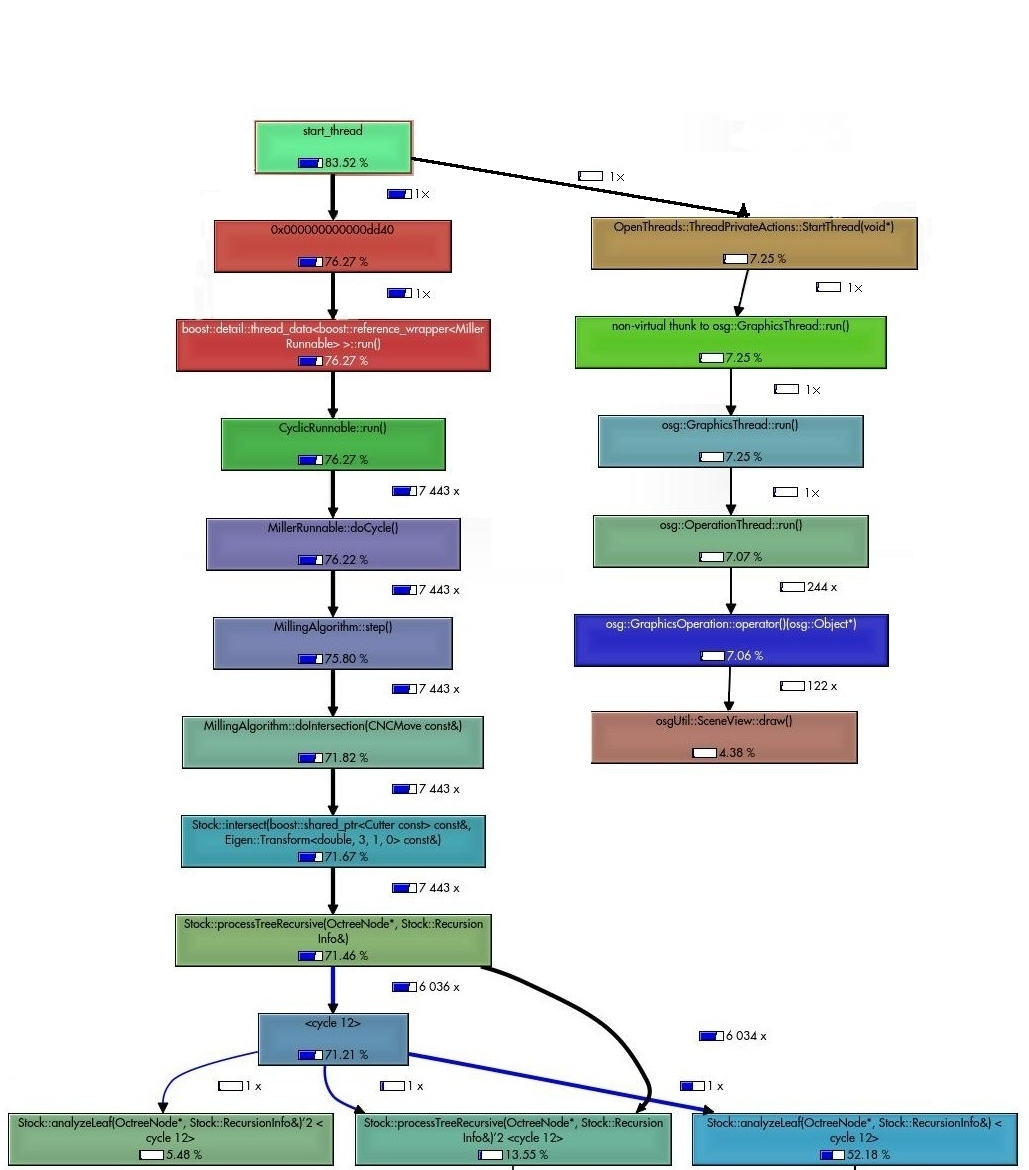
\includegraphics[width=.97\textwidth]{./img/callgraph.jpg}
	\caption{Grafico delle chiamate del simulatore.}
	\label{fig:callgraph}
\end{figure}

Il modulo che lavora per la maggior parte del tempo è chiaramente il Miller, che consuma circa i 3/4 di cicli processore impiegati in totale. Il metodo \texttt{CyclicRunnable::run()} chiama infatti \texttt{MillerRunnable::doCycle()} per 7443 volte, ovvero il numero di iterazioni dell'algoritmo di milling. Questa è chiaramente l'operazione più onerosa eseguita dall'algoritmo, e quella in cui si dovrebbero concentrare eventuali sforzi di ottimizzazione per ottenere un prodotto più performante.

La visualizzazione grafica, che inizia con l'invocazione del metodo \texttt{Display::draw()} è invece responsabile del 15\% circa del tempo di calcolo.

Per quanto riguarda i rimanenti moduli, se il configuratore viene eseguito solo preliminarmente alla lavorazione e con compiti di setup, e ci aspettiamo quindi un impatto limitato sul tempo totale, notiamo invece come in questa prova il Meshing sia assente dal grafo, segno di come anche il suo impatto sia limitato rispetto al Milling, conseguenza dell'efficienza dell'algoritmo Marching Cubes e della bontà della sua implementazione. Segnaliamo tuttavia come questo accada con dimensione minima dei voxel pari a 2: diminuendo la dimensione dei voxel l'impatto dovuto a Marching Cubes aumenta notevolmente, quindi ci aspettiamo di veder comparire anche i metodi del Mesher tra quelli più impattanti sul tempo. Tuttavia, questi test non sono stati effettuati, in quanto l'esecuzione di \texttt{callgrind} rallenta di molto il tempo di esecuzione della simulazione, e una run con voxel più piccoli avrebbe richiesto con ogni probabilità diverse ore prima di giungere al termine.

Come si può facilmente evincere dai risultati appena presentati, i metodi che vengono maggiormente invocati sono quelli che permettono l'interazione tra cutter e Octree. Il metodo in assouto più chiamato è infatti \texttt{CylinderCutter::getDistance()} che misura la distanza tra il cutter (che in tutti i test effettuati era appunto di forma cilindrica) e il voxel più vicino, per determinare se c'è intersezione e quindi rimozione di materiale. Segue, con circa metà invocazioni, la gestione degli smart pointers di Boost e, con poco più di un terzo di chiamate, il metodo \texttt{Stock::IntersectionTester::fastInt()} che esegue i calcoli per determinare se c'è intersezione tra cutter e voxel.
